
\begin{tikzpicture}[line cap=round,line join=round,>=stealth,x=1cm,y=1cm, scale=0.6]
\begin{axis}[
x=1cm,y=1cm,
axis lines=middle,
grid style=dashed,
ymajorgrids=true,
xmajorgrids=true,
xmin=-4,    %Valor mínimo que no sobrepasa la gráfica
xmax=4,     %Valor máximo que no sobrepasa la gráfica
ymin=-2,
ymax=9,
xtick={-4,-3,...,4},    % Etiquetas de los ejes
ytick={-2,-1,...,9}]   
\clip(-4,-2) rectangle (4,9);   % Tamaño del rectangulo de los ejes
\draw[line width=2pt,color= blue,smooth,samples=100,domain=-4:-1.1] plot(\x,{abs((\x-7)/((\x)^2-1)});
\draw[line width=2pt,color= blue,smooth,samples=100,domain=1.2:4] plot(\x,{abs((\x-7)/((\x)^2-1)});
\draw[line width=2pt,color= blue,smooth,samples=100,domain=-0.7:0.7] plot(\x,{abs((\x-7)/((\x)^2-1)});%Función a gráficar
\draw[color= blue] (2,2) node {\Large$f(x) = \abs{\dfrac{x-7}{x^2-1}}$};    % Etiqueta
\end{axis}
\end{tikzpicture}